\chapter{实验研究}

本章主要通过实验来验证所选用硬件组成自动分拣系统的可用性、稳定性和准确定,以及所选用目标检测算法的优越性。然后通过实验
验证深度学习云平台的可用性与稳定性。第一部分将针对自动分拣系统的分拣延时和分拣准确率进行实验,对YOLOv3和YOLOv3-tiny在
自动分拣系统中的延时进行对比与选择。然后对应用YOLOv3-tiny的自动分拣系统的分拣准确率进行实验。第二部分针对深度学习云平台的
Web前端和服务器后端进行了性能稳定性测试。

\section{机械臂分拣系统性能实验}

本节将所设计的基于深度学习的自动分拣系统进行实验,包括图像处理模块的延时实验和分拣准确率实验。其中,延时实验主要是将YOLOv3和YOLOv3-tiny
部署在自动分拣系统后的延时进行对比,从而验证选择YOLOv3-tiny模型配置的优越性。分拣准确率实验又包括
分拣分类准确率实验和抓取成功率实验。前者主要衡量图像处理模块将工件进行准确分类的能力,后者主要衡量图像处理模块识别工件边框
的能力。

本实验中,硬件平台如表\ref{table:exper:hardware}所示。

{
    \begin{table}[htb] 
        \zihao{5}
        \caption{实验各硬件平台配置表}
        \label{table:exper:hardware}
        \centering
        \begin{tabular}[t]{c|c|c|c|c|c}
            \hline
            工件 & 摄像头 & 图像处理平台 & 机械臂 & 显示器 & 服务器  \\
            \hline
            3D打印工件 & 罗技C270 & Jetson TX2 & DOBOT & AOC I2490VXH & DELL T630 \\
            \hline 
        \end{tabular} 
    \end{table}
}

上表所示配置即第二章中所介绍的自动分拣系统的硬件选型配置。实验环境下为自动分拣系统的Jetson TX2配备了显示器,
主要目的为观测目标检测的效果实况,以及记录当前图像处理的FPS。此外,实验环境和实际使用中,Jetson TX2开启最大功耗模式。

软件环境如表\ref{table:exper:software}所示。

{
    \begin{table}[htb] 
        \zihao{5}
        \caption{实验软件环境配置表}
        \label{table:exper:software}
        \centering
        \begin{tabular}[t]{c|c|c|c|c|c}
            \hline
            操作系统 & 模块通信 & G-Code支持 & 算法部署 & 编译工具 & 脚本环境  \\
            \hline
            Linux tegra-ubuntu & USB/ROS/串口 & Marlin固件 & darknet\_ros & catkin\_make & Python/Shell \\
            \hline 
        \end{tabular} 
    \end{table}
}

分拣延时的实验数据通过修改自动分拣系统图像处理模块代码直接将数据保存到本地得到;分拣准确率的实验数据通过人工放置工件和人工观察记录得到。


\subsection{自动分拣系统图像处理模块算法性能试验}

本文第三章第三节中已对YOLOv3和YOLOv3-tiny的性能进行了比较,该比较基于服务器环境,非部署环境。因此本小节将对部署后两者的性能进行对比试验,以
验证针对本任务YOLOv3-tiny配置的优越性。

使用darknet\_ros分别将YOLOv3和YOLOv3-tiny配置的模型部署到自动分拣系统的图像处理模块进行延时实验。实验比较参数为FPS(Frame per Second),即图像处理模块预测图片后显示到显示器
上的帧率。该参数可以反映出图像处理模块进行图像预测的能力,即每秒能够处理的图片数量。实验采集了两个模型部署后处理图片的50个瞬时FPS数据,
数据采集如表\ref{table:delay:data}所示。

{
    \begin{table}[htb] 
        \zihao{5}
        \caption{延时实验数据采集表}
        \label{table:delay:data}
        \centering
        \begin{tabular}[t]{c|c|c|c|c|c|c|c|c|c|c}
            \hline
            \diagbox{配置}{FPS}{编号} & 1 & 2 & 3 & 4 & 5 & 6 & 7 & 8 & 9 & 10 \\
            \hline
            YOLOv3 & 1.51 & 1.48 & 1.49 & 1.53 & 1.56 & 1.50 & 1.54 & 1.55 & 1.40 & 1.48\\
            %%\hline 
            YOLOv3-tiny & 14.92 & 15.20 & 15.49 & 14.65 & 14.90 & 14.78 & 14.56 & 15.50 & 15.18 & 15.04\\
            \hline
            & 11 & 12 & 13 & 14 & 15 & 16 & 17 & 18 & 19 & 20 \\
            \hline
            YOLOv3 & 1.49 & 1.54 & 1.52 & 1.54 & 1.51 & 1.40 & 1.44 & 1.49 & 1.47 & 1.52\\
            %%\hline 
            YOLOv3-tiny & 15.41 & 15.10 & 15.19 & 15.65 & 14.98 & 15.12 & 15.34 & 14.90 & 14.88 & 14.72\\
            \hline
            & 21 & 22 & 23 & 24 & 25 & 26 & 27 & 28 & 29 & 30 \\
            \hline
            YOLOv3 & 1.38 & 1.46 & 1.42 & 1.52 & 1.54 & 1.44 & 1.53 & 1.45 & 1.50 & 1.52\\
            %%\hline 
            YOLOv3-tiny & 15.01 & 15.22 & 15.05 & 15.43 & 14.87 & 15.23 & 15.04 & 14.81 & 14.78 & 14.92\\
            \hline
            & 31 & 32 & 33 & 34 & 35 & 36 & 37 & 38 & 39 & 40 \\
            \hline
            YOLOv3 & 1.49 & 1.50 & 1.56 & 1.42 & 1.50 & 1.41 & 1.43 & 1.53 & 1.55 & 1.51\\
            %%\hline 
            YOLOv3-tiny & 14.91 & 14.92 & 15.32 & 15.51 & 14.85 & 14.66 & 14.94 & 15.20 & 14.68 & 15.15\\
            \hline
            & 41 & 42 & 43 & 44 & 45 & 46 & 47 & 48 & 49 & 50 \\
            \hline
            YOLOv3 & 1.53 & 1.52 & 1.54 & 1.52 & 1.48 & 1.51 & 1.50 & 1.53 & 1.49 & 1.50\\
            %%\hline 
            YOLOv3-tiny & 14.95 & 15.04 & 15.22 & 15.21 & 15.15 & 14.92 & 15.01 & 14.88 & 15.02 & 15.27\\
            \hline
        \end{tabular} 
    \end{table}
}

两个模型瞬时FPS曲线图及平均FPS对比如图\ref{fig:FPS}所示。


\begin{figure}[h]
    \centering
    \subfigure[瞬时FPS曲线图]{
        \label{fig:FPS:moment}
        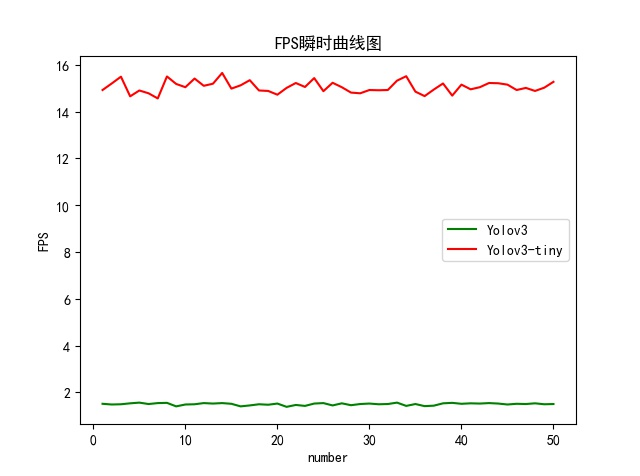
\includegraphics[width=0.46\columnwidth]{pic/chap5/FPS_plot.jpeg}
    }
    \subfigure[平均FPS柱状图]{
        \label{fig:FPS:average}
        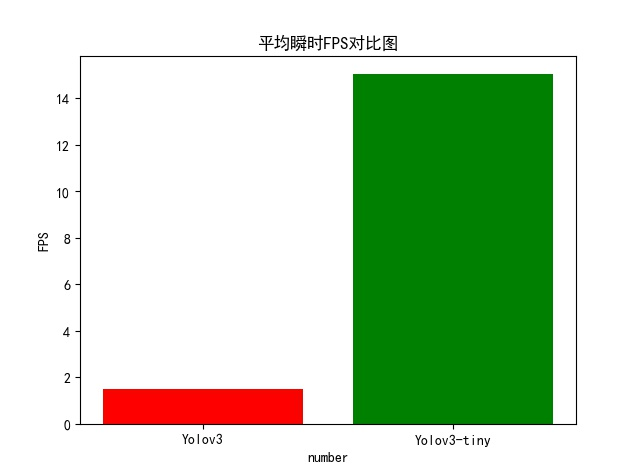
\includegraphics[width=0.46\columnwidth]{pic/chap5/average_FPS_plot.jpeg}
    }
    \caption{YOLOv3和YOLOv3-tiny部署后的FPS对比}
    \label{fig:FPS}
\end{figure}

由数据表及上图可知,YOLOv3部署后的FPS值稳定在1.50附近,平均值为1.4948;YOLOv3-tiny部署后的FPS值稳定在15.0附近,平均值为15.0536。
YOLOv3-tiny的FPS约为YOLOv3的10倍,即YOLOv3-tiny在一秒内能够处理的图片数量十倍于YOLOv3。

此外,实验还比较了两者在实验环境的新数据下的分类准确率。比较参数为51次实验情况下,每个工件的分类准确率。实验数据采集如下表:

{
    \begin{table}[htb] 
        \zihao{5}
        \caption{YOLOv3分类准确率实验数据采集表}
        \label{table:classification:YOLOv3_data}
        \centering
        \begin{tabular}[t]{c|c|c|c|c|c|c|c|c|c|c|c|c|c|c|c|c|c}
            \hline
            \diagbox{模型配置}{实验编号} & 1 & 2 & 3 & 4 & 5 & 6 & 7 & 8 & 9 & 10 & 11 & 12 & 13 & 14 & 15 & 16 & 17\\
            \hline
            dabai是否正确分类 & 1 & 1 & 0 & 1 & 1 & 1 & 1 & 1 & 1 & 1 & 1 & 1 & 1 & 1 & 1 & 1 & 1\\
            fo是否正确分类 & 1 & 1 & 1 & 1 & 1 & 1 & 1 & 1 & 1 & 1 & 1 & 1 & 1 & 1 & 1 & 0 & 1\\
            \hline
            & 18 & 19 & 20 & 21 & 22 & 23 & 24 & 25 & 26 & 27 & 28 & 29 & 30 & 31 & 32 & 33 & 34 \\
            \hline
            dabai是否正确分类 & 1 & 1 & 1 & 1 & 1 & 1 & 1 & 1 & 1 & 0 & 1 & 1 & 1 & 1 & 1 & 1 & 1\\
            fo是否正确分类 & 1 & 1 & 1 & 1 & 1 & 1 & 1 & 1 & 1 & 1 & 1 & 1 & 1 & 1 & 1 & 1 & 1\\
            \hline
            & 35 & 36 & 37 & 38 & 39 & 40 & 41 & 42 & 43 & 44 & 45 & 46 & 47 & 48 & 49 & 50 & 51\\
            \hline
            dabai是否正确分类 & 1 & 1 & 1 & 1 & 1 & 1 & 1 & 1 & 1 & 1 & 1 & 1 & 1 & 1 & 1 & 1 & 1\\
            fo是否正确分类 & 1 & 0 & 1 & 1 & 1 & 1 & 0 & 1 & 1 & 1 & 1 & 1 & 1 & 1 & 1 & 1 & 1\\
            \hline
        \end{tabular}
    \end{table}
}

{
    \begin{table}[htb] 
        \zihao{5}
        \caption{YOLOv3-tiny分类准确率实验数据采集表}
        \label{table:classification:YOLOv3-tiny_data}
        \centering
        \begin{tabular}[t]{c|c|c|c|c|c|c|c|c|c|c|c|c|c|c|c|c|c}
            \hline
            \diagbox{模型配置}{实验编号} & 1 & 2 & 3 & 4 & 5 & 6 & 7 & 8 & 9 & 10 & 11 & 12 & 13 & 14 & 15 & 16 & 17\\
            \hline
            dabai是否正确分类 & 1 & 1 & 0 & 1 & 1 & 1 & 1 & 1 & 1 & 1 & 1 & 1 & 1 & 1 & 0 & 1 & 1\\
            fo是否正确分类 & 1 & 1 & 1 & 1 & 1 & 1 & 1 & 0 & 1 & 1 & 1 & 1 & 1 & 1 & 1 & 1 & 1\\
            \hline
            & 18 & 19 & 20 & 21 & 22 & 23 & 24 & 25 & 26 & 27 & 28 & 29 & 30 & 31 & 32 & 33 & 34 \\
            \hline
            dabai是否正确分类 & 1 & 1 & 1 & 1 & 1 & 1 & 1 & 0 & 1 & 1 & 1 & 1 & 1 & 1 & 1 & 1 & 1\\
            fo是否正确分类 & 1 & 1 & 1 & 1 & 0 & 1 & 1 & 1 & 1 & 1 & 1 & 1 & 1 & 1 & 1 & 0 & 1\\
            \hline
            & 35 & 36 & 37 & 38 & 39 & 40 & 41 & 42 & 43 & 44 & 45 & 46 & 47 & 48 & 49 & 50 & 51\\
            \hline
            dabai是否正确分类 & 1 & 1 & 1 & 1 & 1 & 1 & 1 & 1 & 1 & 1 & 1 & 1 & 1 & 1 & 0 & 1 & 1\\
            fo是否正确分类 & 1 & 1 & 1 & 1 & 1 & 1 & 1 & 1 & 1 & 1 & 1 & 1 & 1 & 1 & 1 & 1 & 1\\
            \hline
        \end{tabular}
    \end{table}
}

表中,1代表正确分类,0代表没有正确分类。分类准确率的计算方式为:
\begin{equation}
    \centering
    \mbox{分类准确率}=\mbox{正确分类样本数}/\mbox{总样本数}
    \label{acc}
\end{equation}

两种模型配置的正确分类数量和分类准确率情况对比如图\ref{fig:classification:compare}所示。

由图可知,YOLOv3的分类准确率略高于YOLOv3-tiny,但两者相差不大,而YOLOv3-tiny部署在Jetson TX2后的图像处理性能十倍于YOLOv3,因此针对本自动分拣系统,
YOLOv3-tiny的模型配置具备相当的优越性,本文最终也选定YOLOv3-tiny作为最终部署在自动分拣系统当中的目标检测算法的模型配置。

\begin{figure}[h]
    \centering
    \subfigure[YOLOv3和YOLOv3-tiny分类情况]{
        \label{fig:classification:num}
        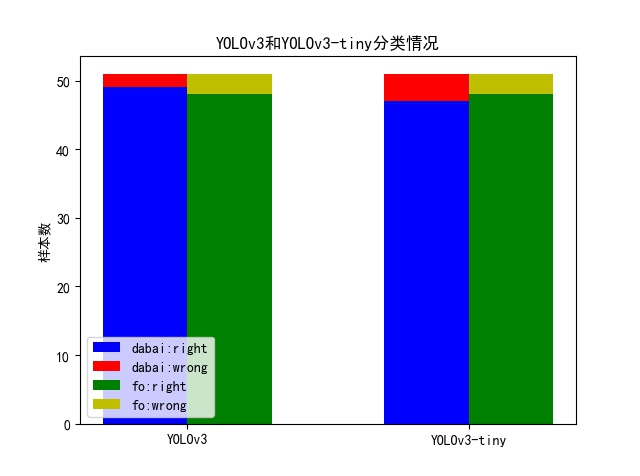
\includegraphics[width=0.46\columnwidth]{pic/chap5/classification_num.jpeg}
    }
    \subfigure[YOLOv3和YOLOv3-tiny分类准确率对比]{
        \label{fig:classification:acc}
        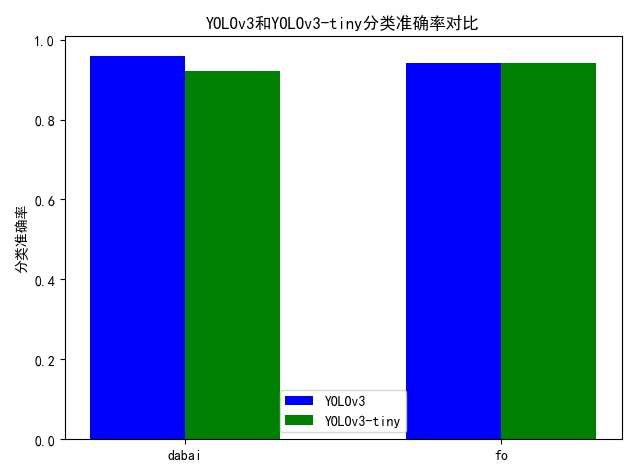
\includegraphics[width=0.46\columnwidth]{pic/chap5/classification_acc.jpeg}
    }
    \caption{YOLOv3和YOLOv3-tiny部署后的分类性能对比}
    \label{fig:classification:compare}
\end{figure}



\subsection{自动分拣系统分拣性能实验}

采用YOLOv3-tiny模型配置作为自动分拣系统图像处理模块的目标检测算法的配置进行部署,具体配置参数见表\ref{table:model:config}。
本小节将对自动分拣系统的分拣性能进行实验。分拣性能评估的是自动分拣系统能够成功抓取工件并将其正确分类的能力。因此,本实验将评估
两个实验数据:抓取成功率和分拣成功率。其中,分拣成功代表自动分拣系统将工件抓取到了正确的位置。即,抓取成功不代表分拣成功,而分拣成功代表一定抓取成功。
分拣成功率是更加严格的评估指标。抓取成功率代表自动分拣系统识别工件边框的准确能力,分拣成功率代表自动分拣系统的功能实现准确率。两者的计算方式如下:
$$\mbox{抓取成功率}=\mbox{机械臂成功抓取样本数}/\mbox{总样本数}$$
\begin{equation}
    \centering
    \mbox{分拣成功率}=\mbox{成功抓取到正确位置的样本数}/\mbox{总样本数}
    \label{fenjian}
\end{equation}

分别将两种工件dabai和fo放置在自动分拣系统的摄像头下,观测其抓取情况,记录其抓取成功和分拣成功的情况。
其中,工件dabai的数据记录表如表\ref{table:fenjian:dabai}所示;
工件fo的数据记录表如表\ref{table:fenjian:fo}所示。

{
    \begin{table}[htb] 
        \zihao{5}
        \caption{针对工件dabai的分拣性能实验数据记录表}
        \label{table:fenjian:dabai}
        \centering
        \begin{tabular}[t]{c|c|c|c|c|c|c|c|c|c|c|c|c|c|c|c|c|c}
            \hline
            \diagbox{参数}{实验编号} & 1 & 2 & 3 & 4 & 5 & 6 & 7 & 8 & 9 & 10 & 11 & 12 & 13 & 14 & 15 & 16 & 17\\
            \hline
            是否成功抓取 & 1 & 1 & 1 & 0 & 1 & 1 & 1 & 1 & 1 & 1 & 1 & 1 & 1 & 1 & 1 & 0 & 1\\
            是否正确分拣 & 1 & 1 & 1 & 0 & 1 & 1 & 1 & 1 & 1 & 1 & 1 & 1 & 1 & 1 & 0 & 0 & 1\\
            \hline
            & 18 & 19 & 20 & 21 & 22 & 23 & 24 & 25 & 26 & 27 & 28 & 29 & 30 & 31 & 32 & 33 & 34 \\
            \hline
            是否成功抓取 & 1 & 1 & 1 & 1 & 1 & 1 & 1 & 1 & 1 & 1 & 1 & 1 & 1 & 1 & 1 & 1 & 1\\
            是否正确分拣 & 1 & 1 & 1 & 1 & 1 & 1 & 1 & 1 & 1 & 1 & 1 & 1 & 1 & 1 & 1 & 1 & 1\\
            \hline
            & 35 & 36 & 37 & 38 & 39 & 40 & 41 & 42 & 43 & 44 & 45 & 46 & 47 & 48 & 49 & 50 & 51\\
            \hline
            是否成功抓取 & 1 & 1 & 1 & 1 & 1 & 1 & 1 & 1 & 1 & 1 & 1 & 1 & 1 & 1 & 1 & 1 & 1\\
            是否正确分拣 & 1 & 1 & 1 & 1 & 1 & 1 & 1 & 1 & 1 & 1 & 1 & 0 & 1 & 1 & 1 & 1 & 1\\
            \hline
        \end{tabular}
    \end{table}
}

{
    \begin{table}[htb] 
        \zihao{5}
        \caption{针对工件fo的分拣性能实验数据记录表}
        \label{table:fenjian:fo}
        \centering
        \begin{tabular}[t]{c|c|c|c|c|c|c|c|c|c|c|c|c|c|c|c|c|c}
            \hline
            \diagbox{参数}{实验编号} & 1 & 2 & 3 & 4 & 5 & 6 & 7 & 8 & 9 & 10 & 11 & 12 & 13 & 14 & 15 & 16 & 17\\
            \hline
            是否成功抓取 & 1 & 1 & 1 & 1 & 1 & 1 & 1 & 1 & 1 & 1 & 1 & 1 & 1 & 0 & 1 & 1 & 1\\
            是否正确分拣 & 1 & 1 & 1 & 1 & 1 & 1 & 1 & 1 & 1 & 1 & 1 & 0 & 1 & 0 & 1 & 1 & 1\\
            \hline
            & 18 & 19 & 20 & 21 & 22 & 23 & 24 & 25 & 26 & 27 & 28 & 29 & 30 & 31 & 32 & 33 & 34 \\
            \hline
            是否成功抓取 & 1 & 1 & 0 & 1 & 1 & 1 & 1 & 1 & 1 & 0 & 1 & 1 & 1 & 1 & 1 & 1 & 1\\
            是否正确分拣 & 1 & 0 & 0 & 1 & 1 & 1 & 1 & 1 & 1 & 0 & 1 & 1 & 1 & 1 & 1 & 1 & 1\\
            \hline
            & 35 & 36 & 37 & 38 & 39 & 40 & 41 & 42 & 43 & 44 & 45 & 46 & 47 & 48 & 49 & 50 & 51\\
            \hline
            是否成功抓取 & 1 & 1 & 1 & 1 & 1 & 1 & 1 & 1 & 1 & 1 & 1 & 1 & 1 & 1 & 1 & 1 & 1\\
            是否正确分拣 & 1 & 1 & 1 & 1 & 1 & 1 & 1 & 1 & 1 & 1 & 1 & 1 & 1 & 1 & 1 & 1 & 1\\
            \hline
        \end{tabular}
    \end{table}
}

两种工件的抓取成功率和分拣成功率计算如表\ref{table:fenjian:res}所示。由表可知,自动分拣系统的抓取成功率在95\%左右,
更为严格的分拣成功率则在91\%左右。基本达到可投入使用的水平。 

{
    \begin{table}[htb] 
        \zihao{5}
        \caption{分拣性能实验数据计算结果}
        \label{table:fenjian:res}
        \centering
        \begin{tabular}[t]{ccc}
            \hline
            工件 & 抓取成功率 & 分拣成功率\\
            \hline
            dabai & 96.08\% & 92.16\% \\
            fo & 94.12\% & 90.20\% \\
            \hline
        \end{tabular}
    \end{table}
}



\section{基于深度学习的目标检测模型云平台性能测试}
 
\subsection{Web前端性能测试实验}  
 
在基于深度学习的目标检测模型训练云平台中,
Web前端承担着与用户交互的任务,其性能表现好坏将直接影响用户使用的体验。本小节对Web前端页面的网络收发、页面渲染、js性能等进行测试,测试环境如表\ref{table:Web:env}所示。

{
    \begin{table}[htb]   
        \zihao{5}
        \caption{Web前端性能测试环境}
        \label{table:Web:env}
        \centering
        \begin{tabular}[t]{ccccc}
            \hline
            设备 & 操作系统 & CPU & 内存 & 浏览器\\
            \hline
            Macbook Pro 2018 & macOS & 8核 2.2GHZ & 16GB & safari \\
            \hline
        \end{tabular}
    \end{table}
}

将safari的开发选项调至菜单栏,使用其时间线录制工具,录制深度学习云平台Home界面的接收和渲染情况。
实验结果如图\ref{fig:web:test}所示。
由图可以看出,深度学习云平台的Web页面网络收发用时在2ms以内,页面渲染用时在4ms以内,js响应用时在30ms以内。收发数据量大小为250KB左右
,其中只有1.8KB没有被缓存,即第二次访问云平台网站时,只需要接收1.8KB的网络数据。可以看出,云平台的Web前端页面
的各项性能均非常优异。这种优异的性能主要来源于Bootstrap框架的优化和云平台页面本身的简洁性。

\begin{figure}[t]
    \centering
    \subfigure[前端页面网络收发耗时情况]{
        \label{fig:web:net}
        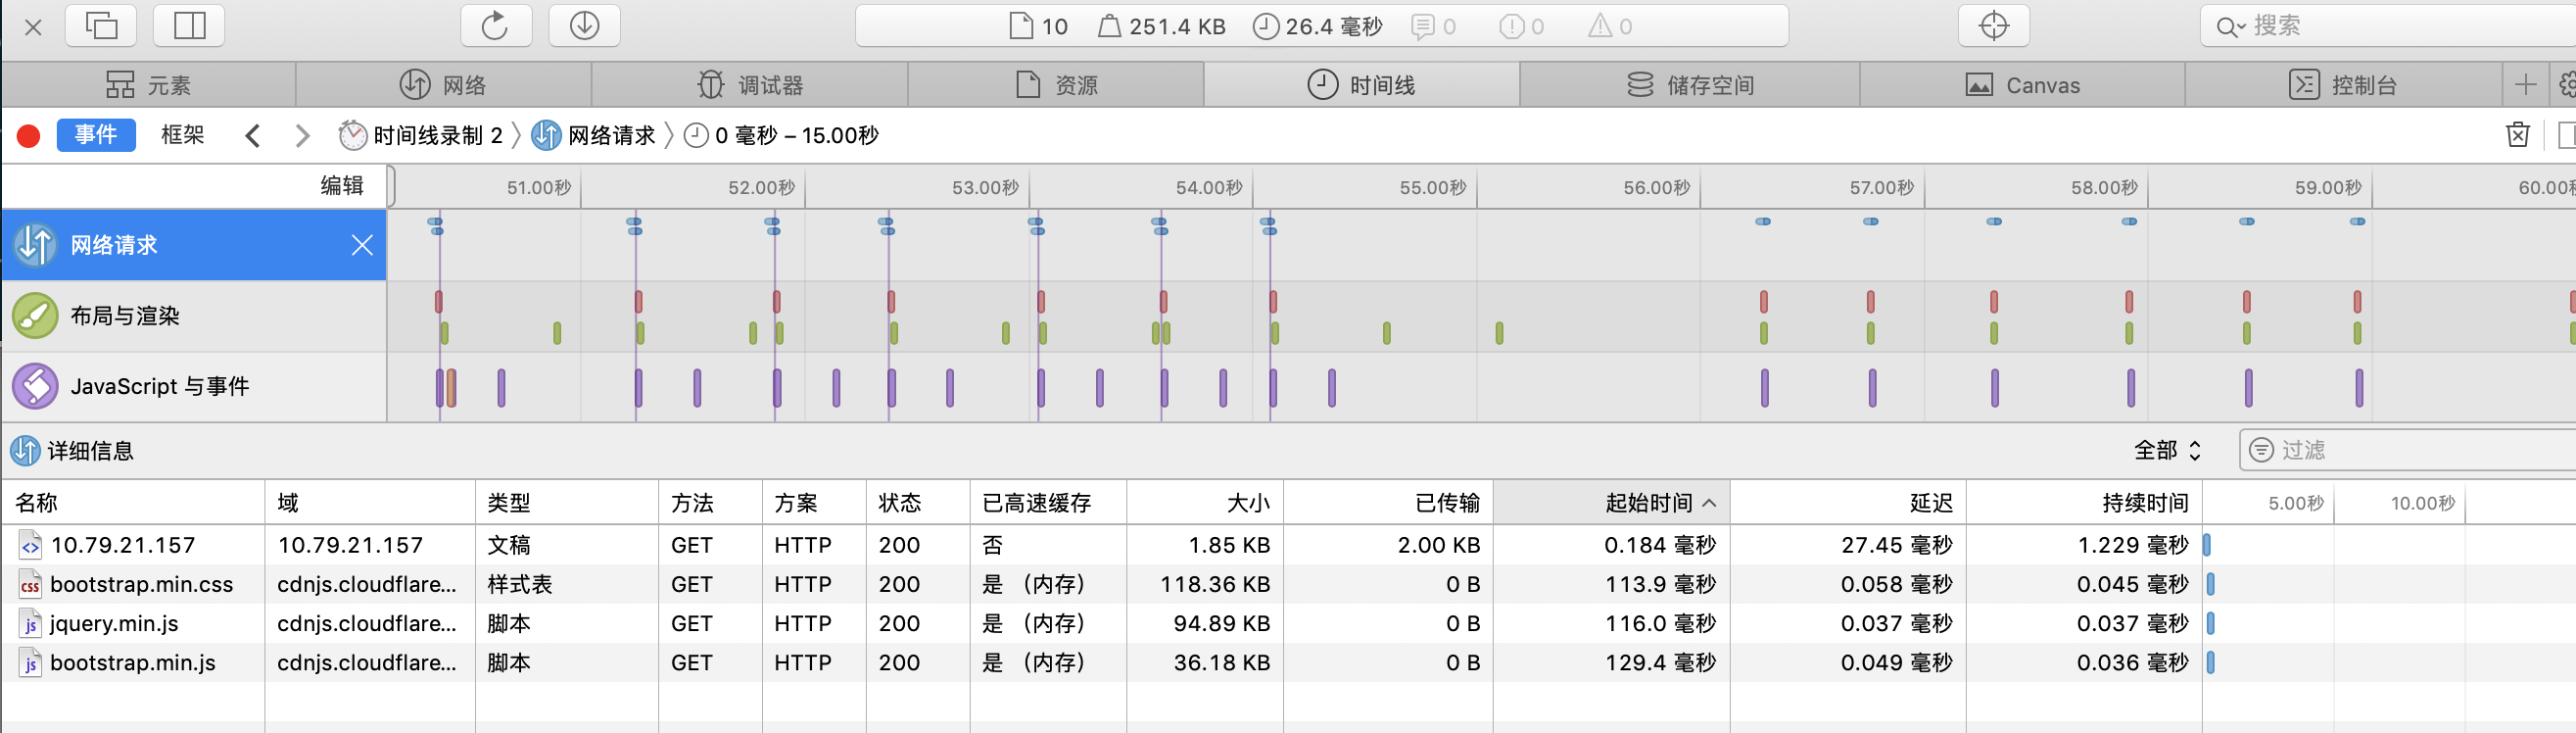
\includegraphics[width=\textwidth]{pic/chap5/web_net.png}
    }
    \subfigure[前端页面渲染耗时情况]{
        \label{fig:web:css}
        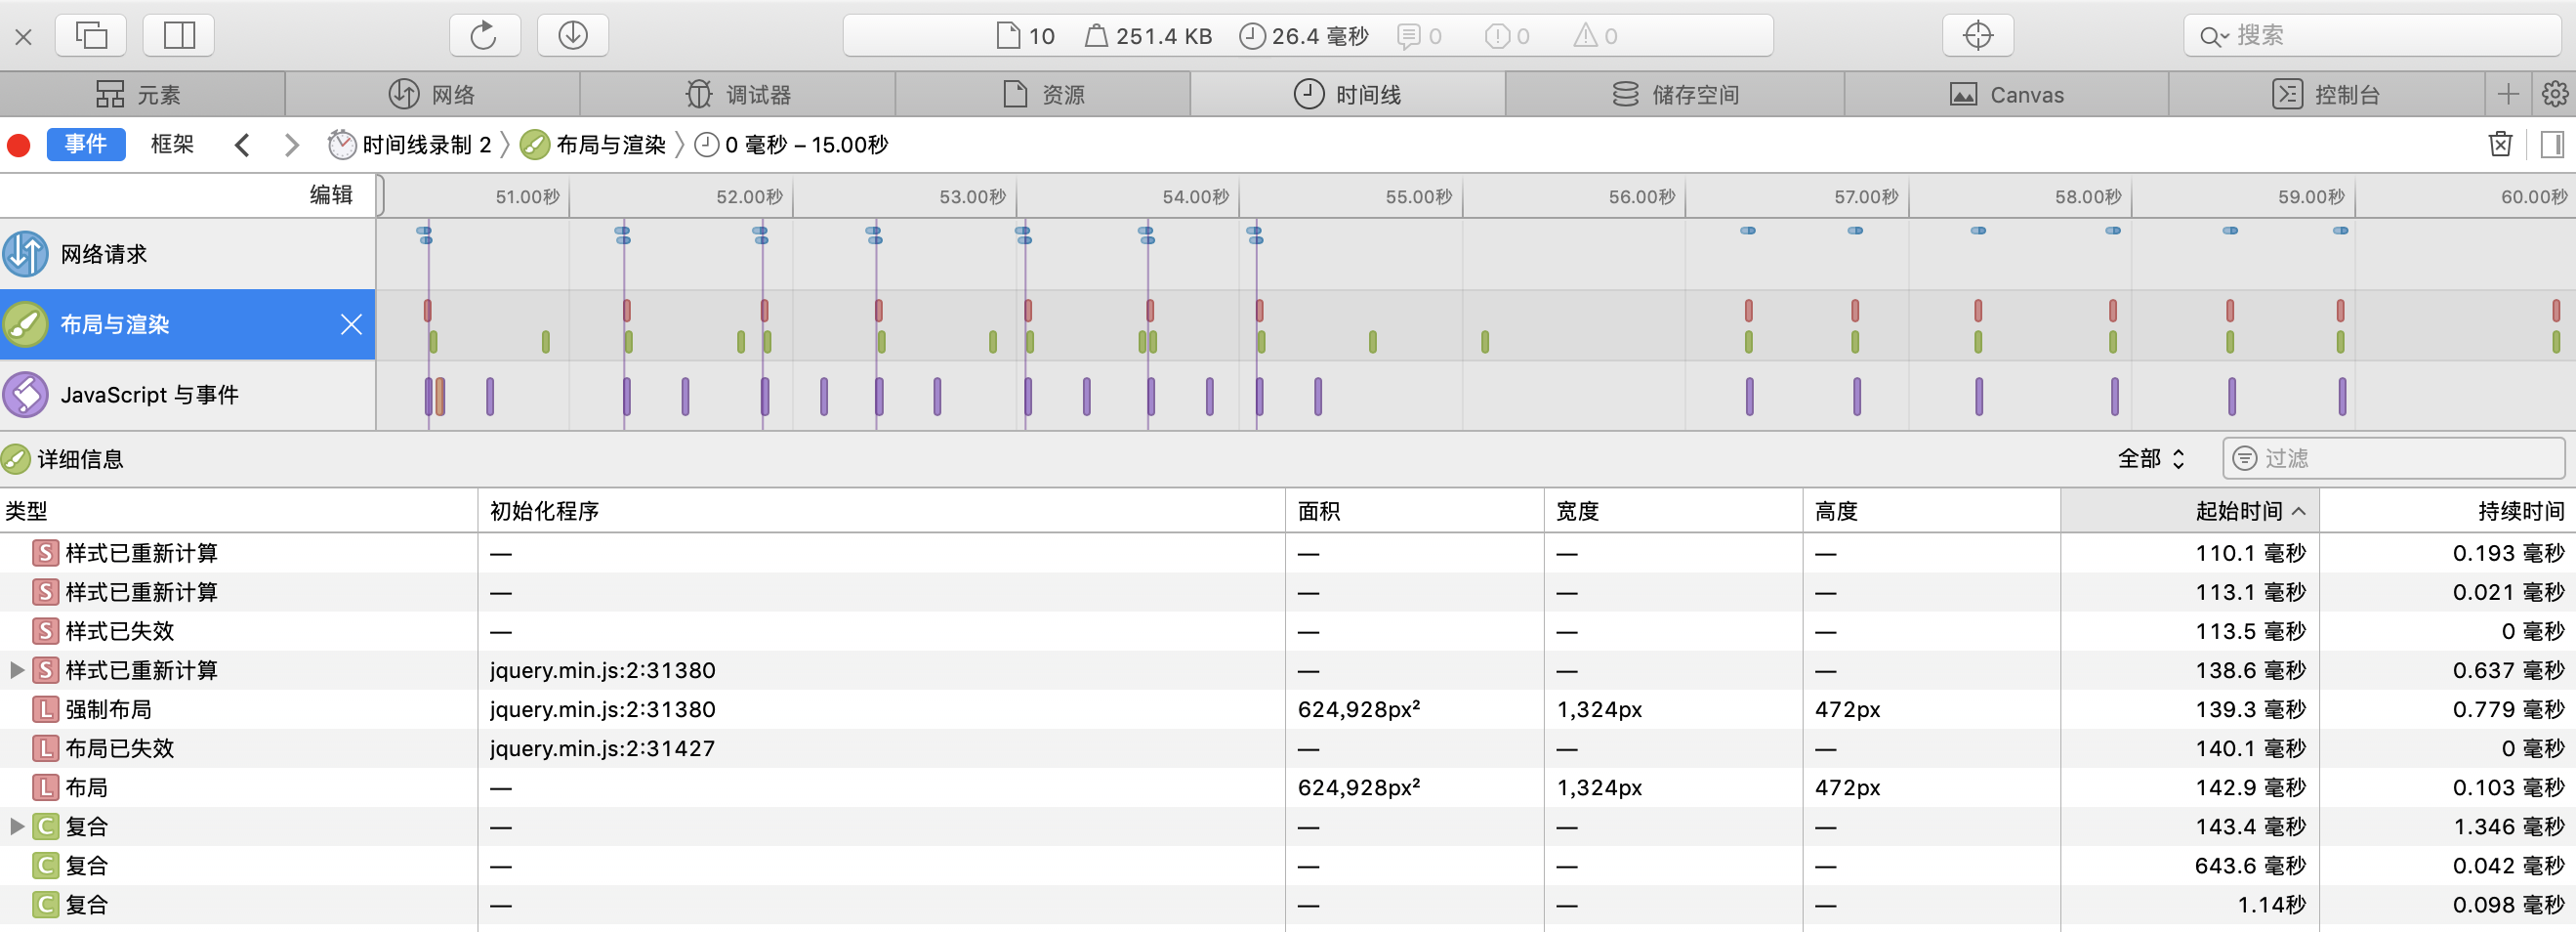
\includegraphics[width=\textwidth]{pic/chap5/web_css.png}
    }
    \subfigure[前端页面js响应耗时情况]{
        \label{fig:web:js}
        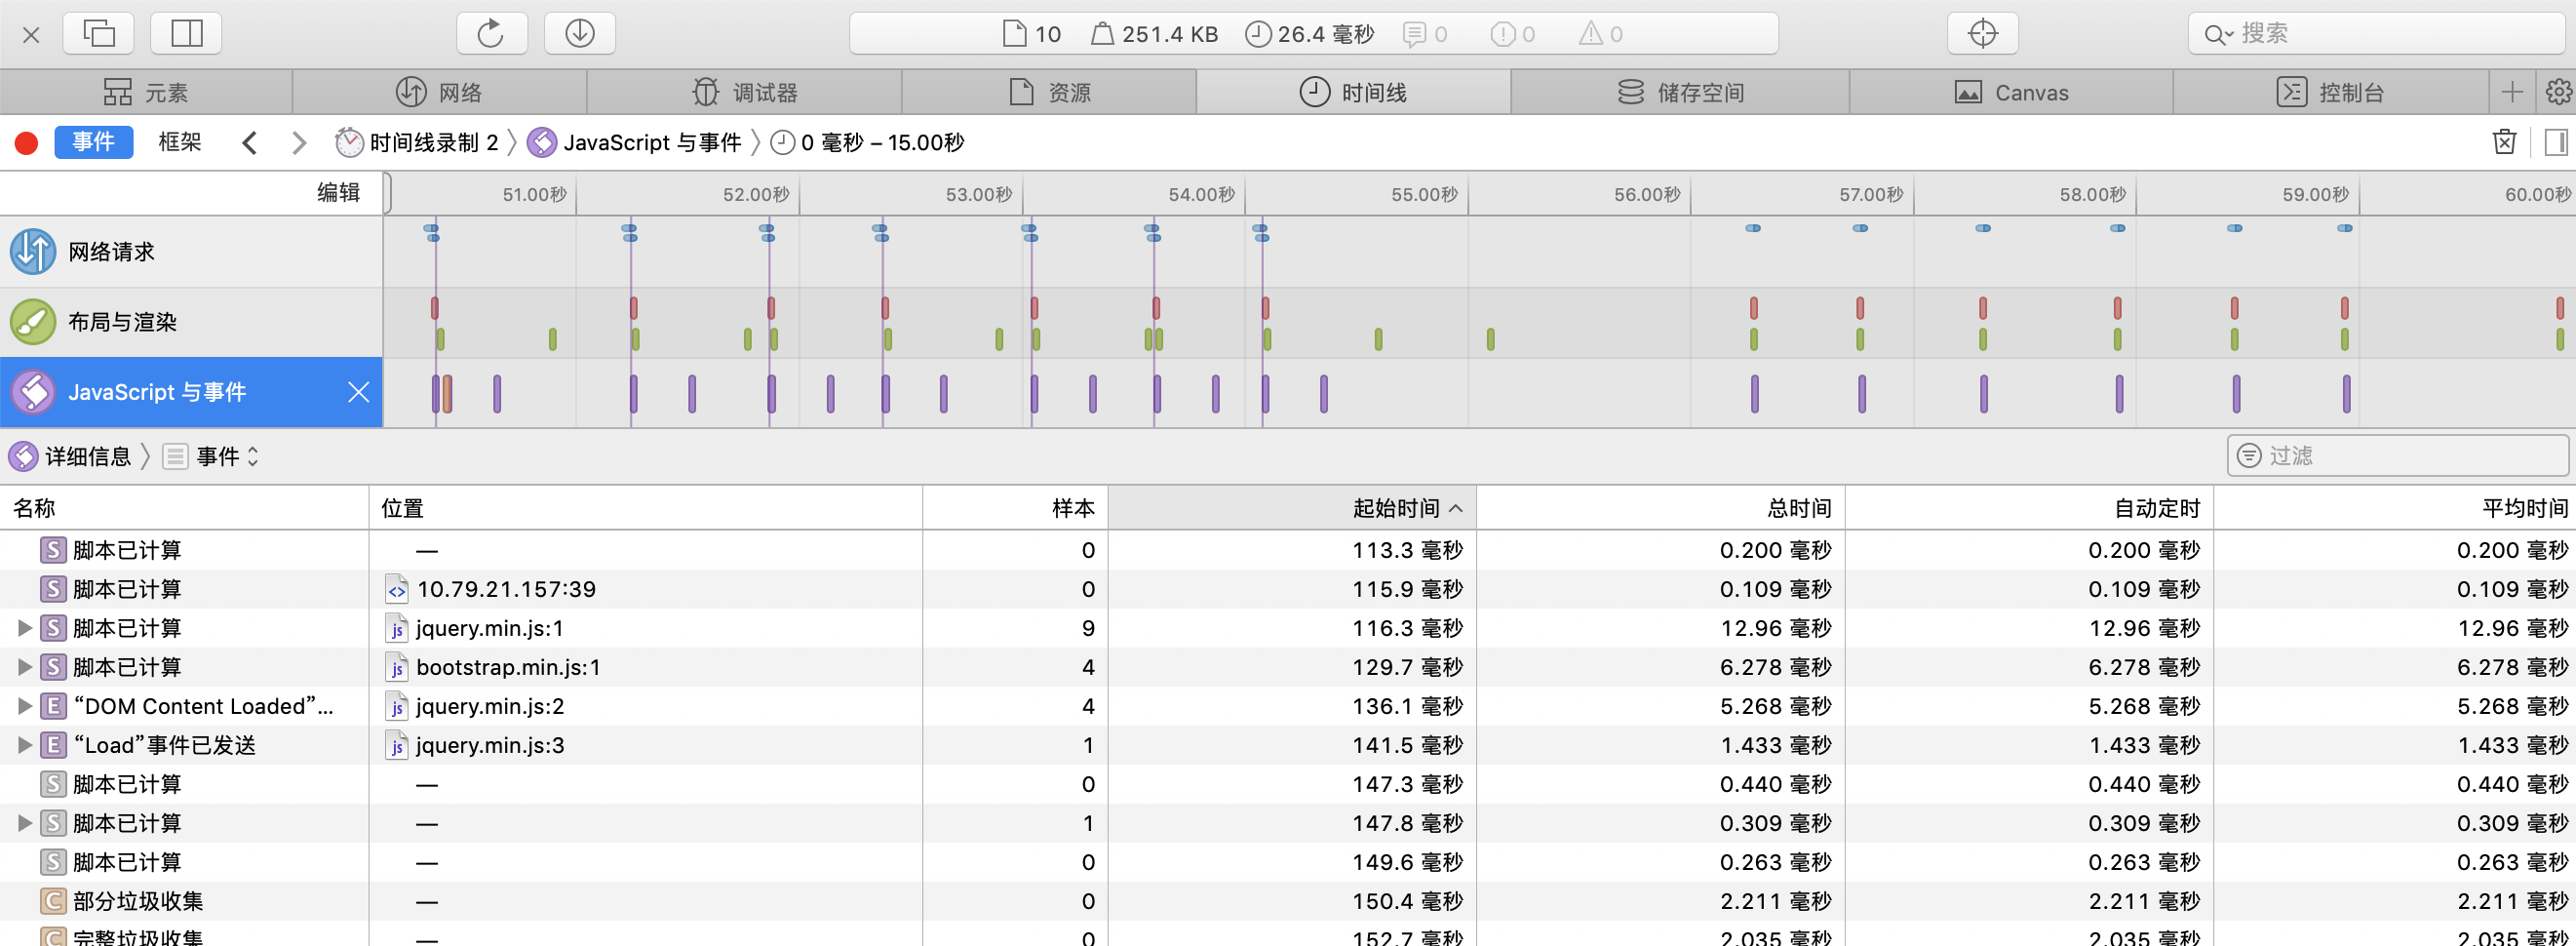
\includegraphics[width=\textwidth]{pic/chap5/web_js.png}
    }
    \caption{前端性能测试实验}
    \label{fig:web:test}
\end{figure}


\subsection{服务器端性能测试实验}

深度学习云平台的服务端服务于每个使用云平台的用户,其性能同样影响着用户体验。深度学习云平台所使用服务器配置如表\ref{table:server:config}。
测试用客户端参数如表\ref{table:Web:env}所示。本小节将对深度学习云平台服务端进行压力测试,
测试其承载能力。主要关注参数为能够同时承载的用户数量、服务器响应耗时等。

本实验使用Locust\cite{locust}为工具进行服务器压力测试实验。其参数设置如表\ref{table:locust:param}所示。在本次实验中,我们测试了5000个用户
同时使用云平台的情况。具体模拟情况为:用户数从0开始,每秒增加20个用户,每个用户的模拟行为为访问云平台主页一次和点击两次开始训练按钮,
每个用户的每次行为之间的间隔为5-15s之间的随机数。测试请求采用的通信协议为HTTP通信协议,访问云平台主页为GET请求方法,点击开始训练按钮为POST请求方法。
测试的链接即云平台网站域名:http://10.79.21.157:5000。
测试客户端与云平台服务器同处于校园局域网下,其IP地址为ZJUWLAN所分配的动态IP地址。

{
    \begin{table}[htb]   
        \zihao{5}
        \caption{Locust测试环境参数}
        \label{table:locust:param}
        \centering
        \begin{tabular}[t]{cccc}
            \hline
            用户数 & 每秒产生用户数 & 用户行为 & 用户行为间隔 \\
            \hline
            5000 & 20 & 访问主页1次+点击按钮2次  & random(5-15s) \\
            \hline
        \end{tabular}
    \end{table}
}

Locust测试时的GUI界面如图\ref{fig:locust:gui}所示,由图可知,访问云平台Home界面时接收数据量为1891byte,主要为Home界面的html文件数据;点击开始训练按钮
接收数据量为17byte,为服务器返回的确认信息和状态码。实验的汇总数据如表\ref{table:locust:data}所示。本次实验共持续337s,共发送请求92726个,其中有30944个
GET请求,61782个POST请求。最短耗时与最长耗时差距极大,说明实验后期随着用户数量增加,并发数上升,出现了一些高延时请求,服务器请求响应性能发生震荡。

{
    \begin{table}[htb]   
        \zihao{5}
        \caption{服务器压力测试数据汇总表(耗时单位均为ms)}
        \label{table:locust:data}
        \centering
        \begin{tabular}[t]{cccccccc}
            \hline
            名称 & 请求数 & 失败数 & 平均耗时 & 最短耗时 & 最长耗时 & 耗时中位数 & 请求数/s \\
            \hline
            GET \quad / & 30944 & 0(0.00\%) & 1059 & 7 & 48713 & 73 & 121.70 \\
            POST \quad /train & 61782 & 0(0.00\%) & 1062 & 7 & 50290 & 72 & 237.70 \\ 
            \hline
            Total & 92726 & 0(0.00\%) & & & & & 359.40 \\
            \hline
        \end{tabular}
    \end{table}
}



\begin{figure}[h]
    \centering
    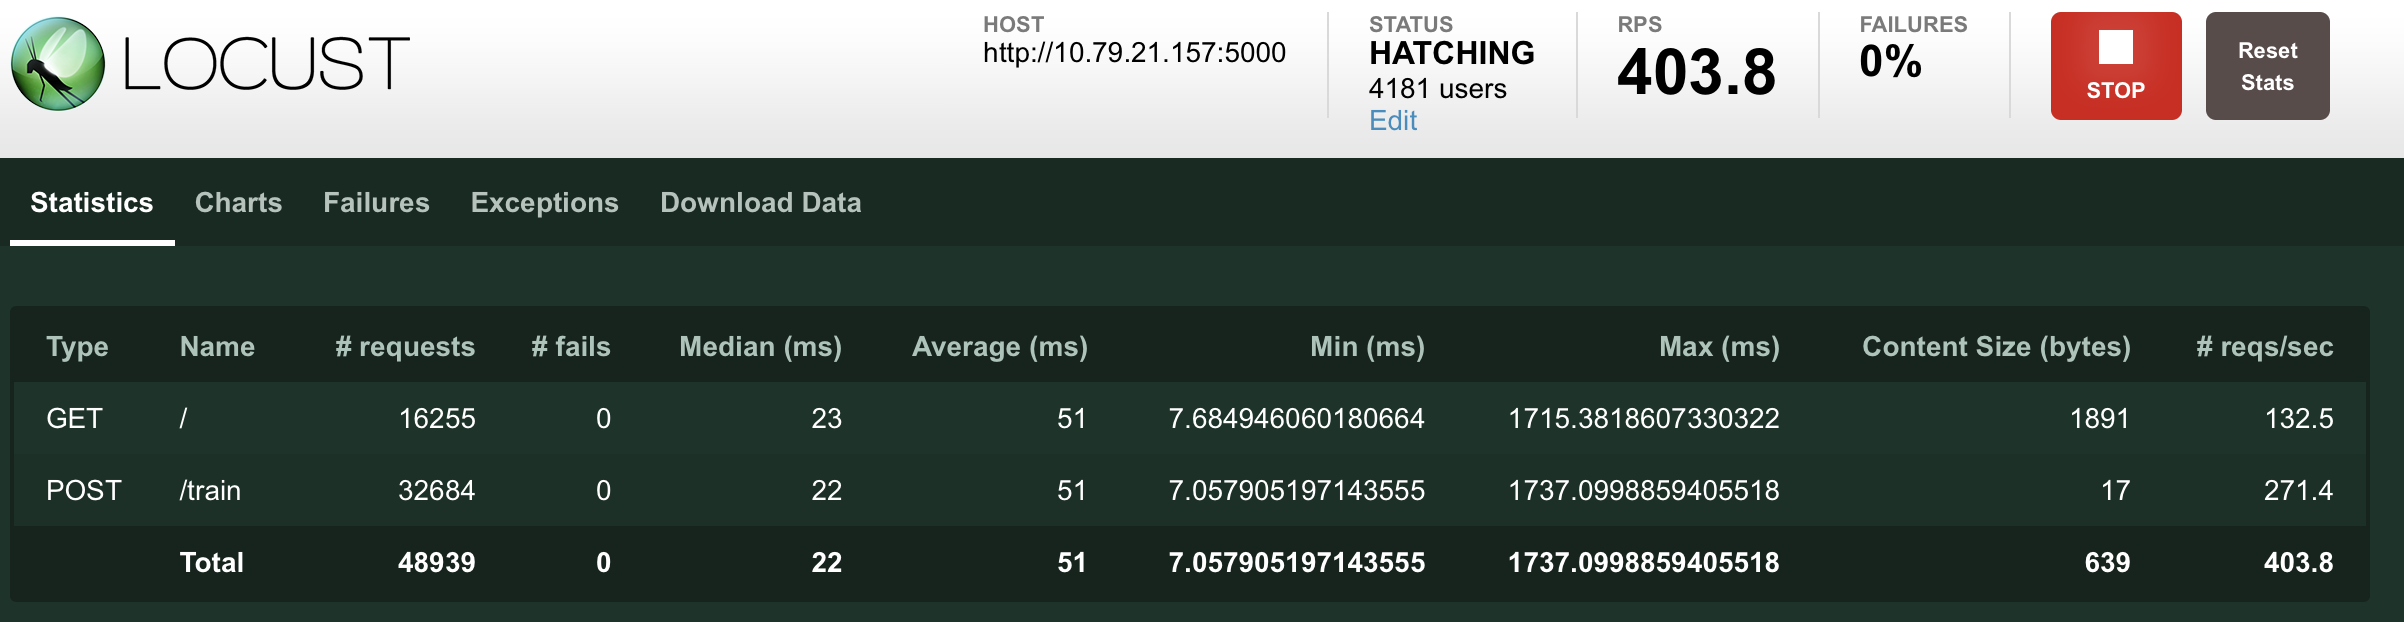
\includegraphics[width=\textwidth]{pic/chap5/Locust_test.png}
    \caption{Locust GUI界面}
    \label{fig:locust:gui}
\end{figure}

如图\ref{fig:locust:rps}为实验期间,每秒请求数(RPS)随时间的变化曲线。实验前期,用户量较少,随着用户数的增加,RPS逐渐增加。
12:29:12之后,RPS发生大幅震荡,说明随着用户数的增加,一些用户发送的请求延时变高,阻止了这些用户后续的请求发送。

如图\ref{fig:locust:rt}为实验期间,响应时间随时间的变化曲线。其中,绿色曲线为所有请求耗时的中位数随时间的变化曲线,黄色曲线为所有
请求耗时从大到小排列5\%分位数随时间的变化曲线。前者代表了服务器响应请求的网络传输性能,后者代表了服务器承载多用户数量的并发能力。由图
可知,12:29:12之后,黄色曲线大幅度上升并开始震荡,绿色曲线小幅度上升。说明随着用户数的增加,并发量的增大,一些请求的耗时大大增加,服务的
承载能力到了瓶颈。

如图\ref{fig:locust:user}为实验期间,用户数随时间的变化曲线。按照每秒增加20个用户,5000封顶的设定,用户数到5000便不再增加。根据前面
两幅图的分析可知,服务器在12:29:12后达到性能瓶颈,即用户数达到4000时,服务器性能达到瓶颈。由此可得出结论,本文设计的深度学习云平台,其服务器
可承载4000位用户的同时在线。

实验期间,还使用脚本记录了服务器的CPU使用情况,如图\ref{fig:server:cpu}所示。user曲线为运行服务器驻留程序的用户态CPU使用情况,idle为服务器CPU
的空闲程度。由图可知,实验期间,随着用户数量的增加,服务器CPU的使用稍微增加,但影响不大。因此,服务器的处理能力足够,主要瓶颈发生在网络I/O口和
负载均衡。

由于服务器GPU数量有限,实际使用过程中,无法为大量用户提供计算服务。若希望提高用户覆盖面,则需要加配GPU,使用服务器集群的形式。同时使用负载均衡
来处理大规模并发请求的问题。

\begin{figure}[h]
    \centering
    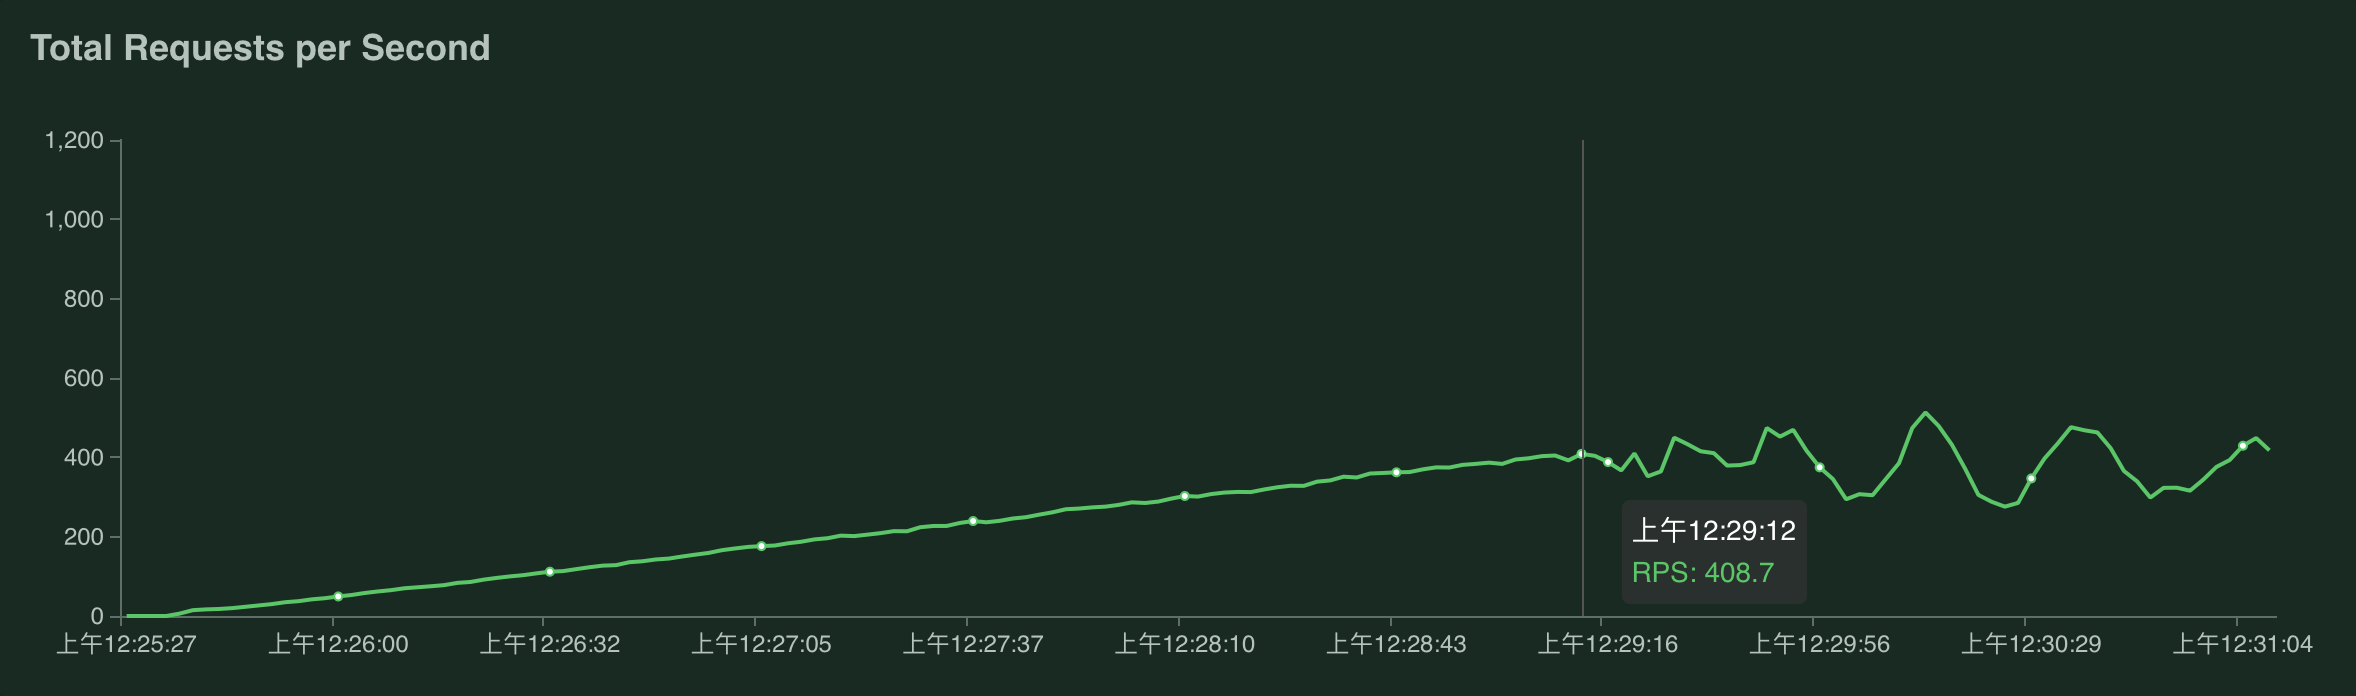
\includegraphics[width=\textwidth]{pic/chap5/rsp.png}
    \caption{每秒请求数随时间的变化曲线}
    \label{fig:locust:rps}
\end{figure}

\begin{figure}[h]
    \centering
    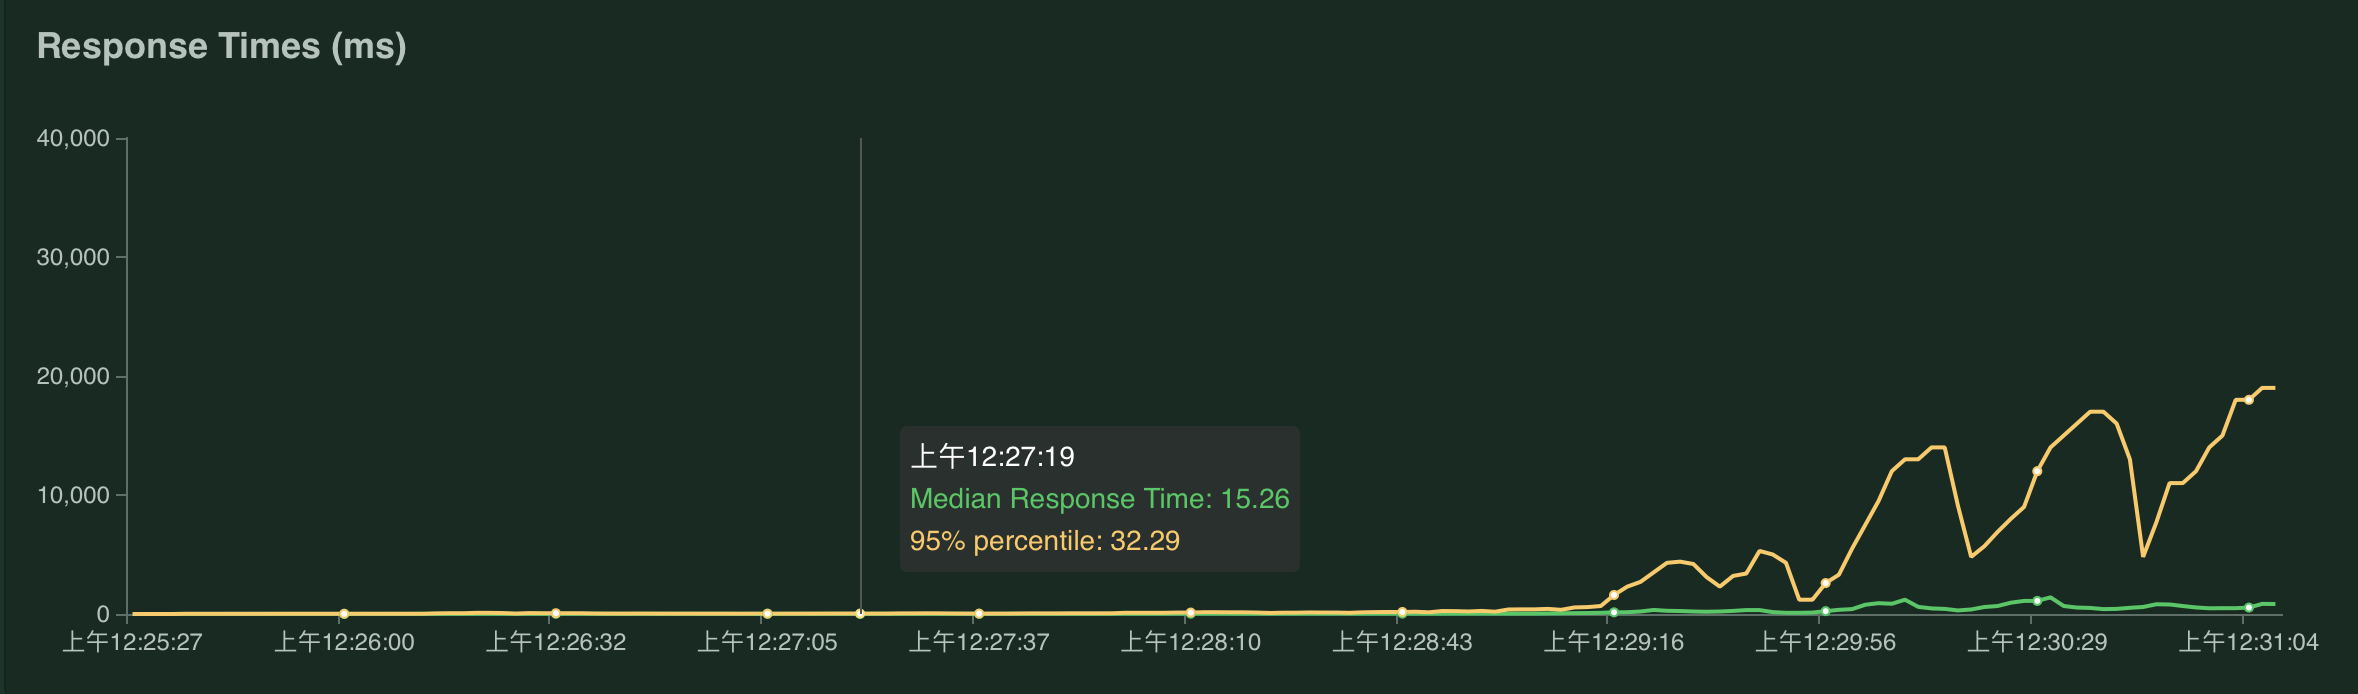
\includegraphics[width=\textwidth]{pic/chap5/rt.png}
    \caption{请求响应耗时随时间的变化曲线}
    \label{fig:locust:rt}
\end{figure}

\begin{figure}[h]
    \centering
    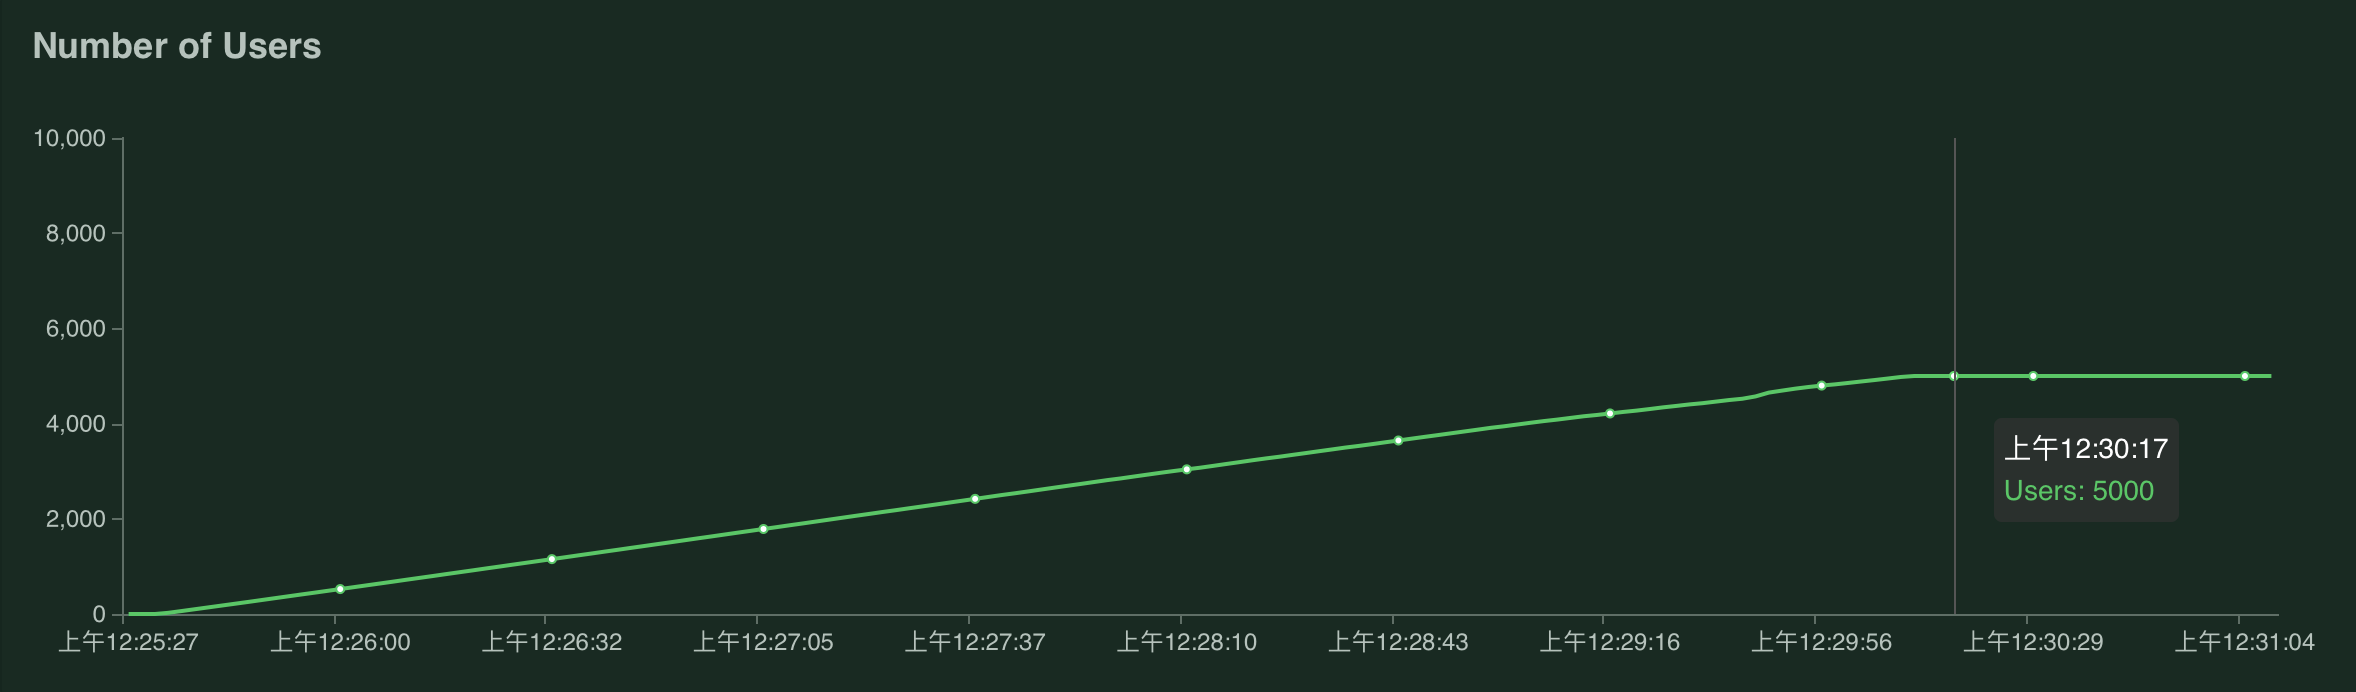
\includegraphics[width=\textwidth]{pic/chap5/user_numbers.png}
    \caption{用户数随时间的变化曲线}
    \label{fig:locust:user}
\end{figure}

\begin{figure}[h]
    \centering
    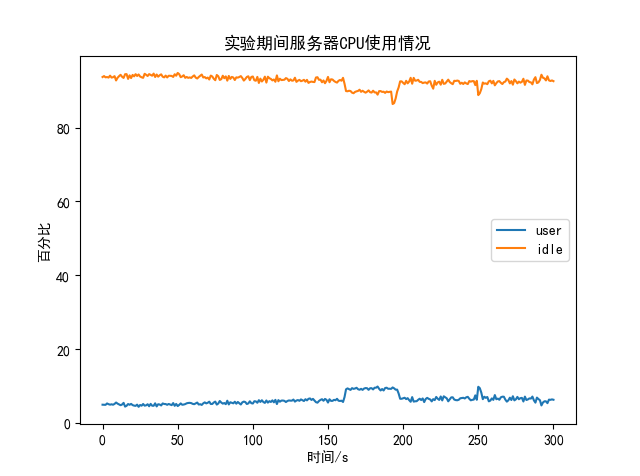
\includegraphics[width=\textwidth]{pic/chap5/server_cpu.png}
    \caption{实验期间服务器CPU使用变化情况}
    \label{fig:server:cpu}
\end{figure}


\section{本章小结}

本章主要对本文设计的两部分系统:自动分拣系统和深度学习训练云平台进行了性能实验。第一节介绍了对自动分拣系统算法选择的
优越性进行了验证,然后验证了本文设计的基于深度学习目标检测算法的自动分拣系统的可用性与准确性。第二节介绍了本文设计开发的
深度学习云平台Web前端和服务器端的可用性与稳定性实验。